%!TEX root = ../swiatlow_thesis.tex
\label{chapter:lhc}

The Large Hadron Collider (LHC) is a 27 km long proton-proton ($pp$) synchotron built on the border of France and Switzerland, near the city of Geneva. The accelerator is nestled beneath mostly bucolic French farmland, as seen in Figure~\ref{fig:lhc:cern-lhc-aerial}. The total costs of the accelerator and the detectors it serves are estimated at \$20 billion, making the LHC one of the largest scientific enterprises ever attempted. \editnote{cite this} The project is full of similar superlatives: the accelerator is the largest machine, the ATLAS detector is the largest detector, the CMS detector is the heaviest. 10,000 scientists from 113 countries work on some aspect of the project, making it one of the best examples of international cooperation that mankind has produced.

%%%%%%%%%%%%%%%%

\begin{figure}
\centering
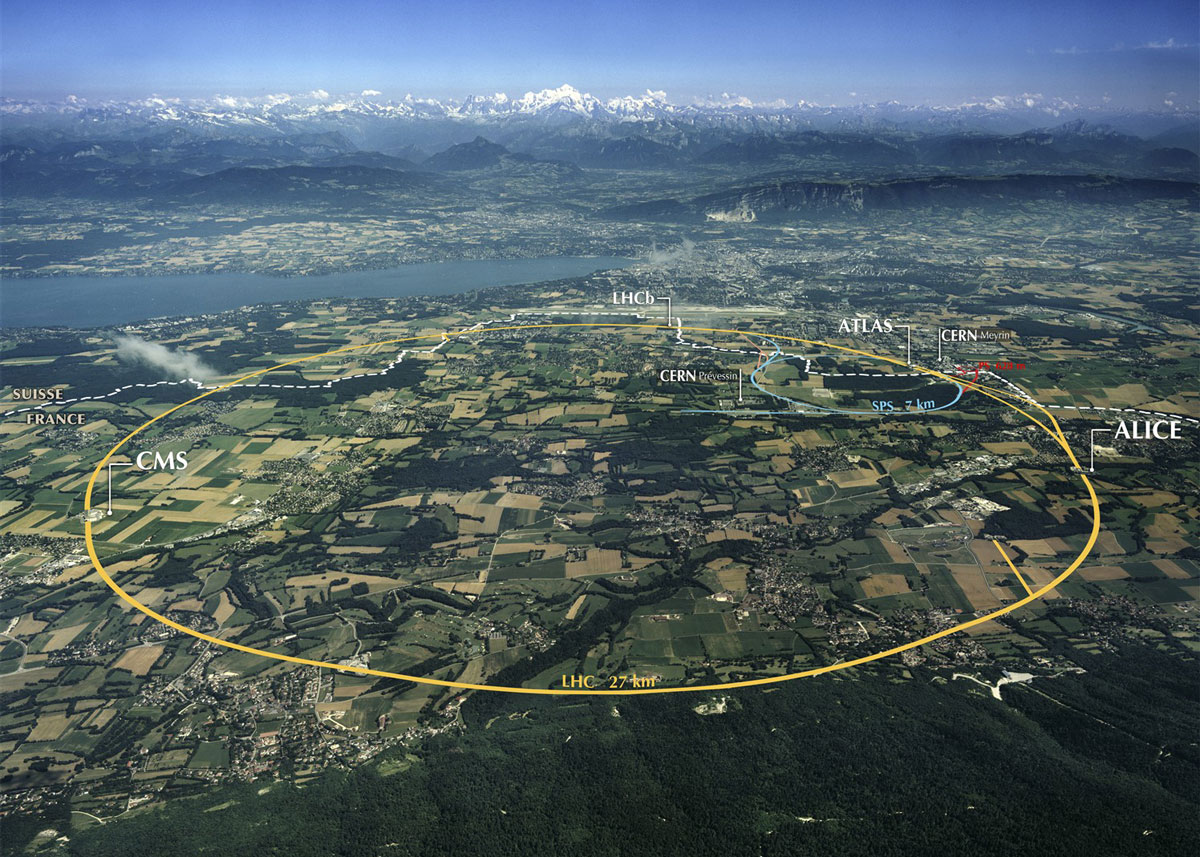
\includegraphics[width=0.8\textwidth]{cern-lhc-aerial.jpg}
\label{fig:lhc:cern-lhc-aerial}
\caption{An aerial view of Geneva, with the location of the LHC superimposed. The individual detectors (described in chapter~\ref{chapter:detector}, as well as the main CERN Meyrin site, are also highlighted. Image courtesy CERN.}
\end{figure}

%%%%%%%%%%%%%%%% 

The design of the machine aims to deliver collisions at $\sqrt{s} = 14$~\TeV~energy at a rate of $10^{34}$~\lumirate-- an energy at which protons in the LHC will be moving at 99.9999991$\%$ the speed of light, and where the beams will contain as much energy as a 38 ton truck traveling at 500 km/h.  As of 2012 collisions had only occured at 8 \TeV and a rate of $5\times10^{33}$~\lumirate-- enough to discover the Higgs Boson, but not yet enough to discover physics beyond the standard model.

The following sections describe first the history of the LHC project, followed by the details of the machine design, luminosity considerations, and operations during 2010-2012.

\section{History}
\label{lhc:history}

The LHC was first discussed publically at the ECFA-CERN Workshop held at Lausanne and Geneva in March of 1984~\cite{ECFA1984}\footnote{4 years and 1 month before the author was born!}. This was a very active time for proposing new collider experiments, as extensive work on the 40~\TeV $pp$ Superconducting Supercollider (to be built in Waxahachie, Texas) had recently displaced a proposal for a 4~\TeV~$p\bar{p}$ Dedicated Collider at Fermilab~\cite{ECFA1984,DC}, though construction continued on Fermilab's 2~\TeV~$p\bar{p}$ Tevatron collider. The Soviet Union was even planning a 6~\TeV~$p\bar{p}$ collider, the Accelerator and Storage Complex (UNK)~\cite{UNK}\editnote{This needs a better citation}. In this busy landscape, the proposal of another machine at CERN-- which was currently building the Large Electron Positron (LEP), the world's largest $e^+/e^-$ collider-- was very ambitious indeed.

Several characteristics made the proposed LHC unique and worth pursuing in such a competitive environment. First, with the construction of the LEP tunnel on track for completion in 1988, the civil-engineering component of the project was greatly reduced, especially compared to the enormous expense of constructing the SSC tunnel. Second, while the design goals of 20~\TeV~collisions were at a significantly lower energy than the SSC, the projected luminosity was eventually designed to be a factor of 10 higher (10$^{34}$~\lumirate, though the initial designs focused on 10$^{33}$~\lumirate) and so the LHC could potentially gain sensitivity by accumulating data more quickly. Finally, as figure \ref{fig:lhc:lep-lhc} shows, the initial designs for the LHC invisaged the LHC beamlines actually sitting on top of the existing LEP beamlines. The resulting hybrid collider would be able to run $pp$, $ep$, and $ee$ collisions. This would not only extend the reach of the physics program by allowing for the study of deep inelastic scattering at higher energies than the HERA collider at DESY \editnote{Cite this-- HERA and $e/p$ if possible.}, but would also allow for the study of $Z$ bosons from $ee$, which could potentially be used as a calibration source for detectors before $pp$ collisions~\cite{ECFA1984}.

%%%%%%%%%%%%%%%%

\begin{figure}
\centering
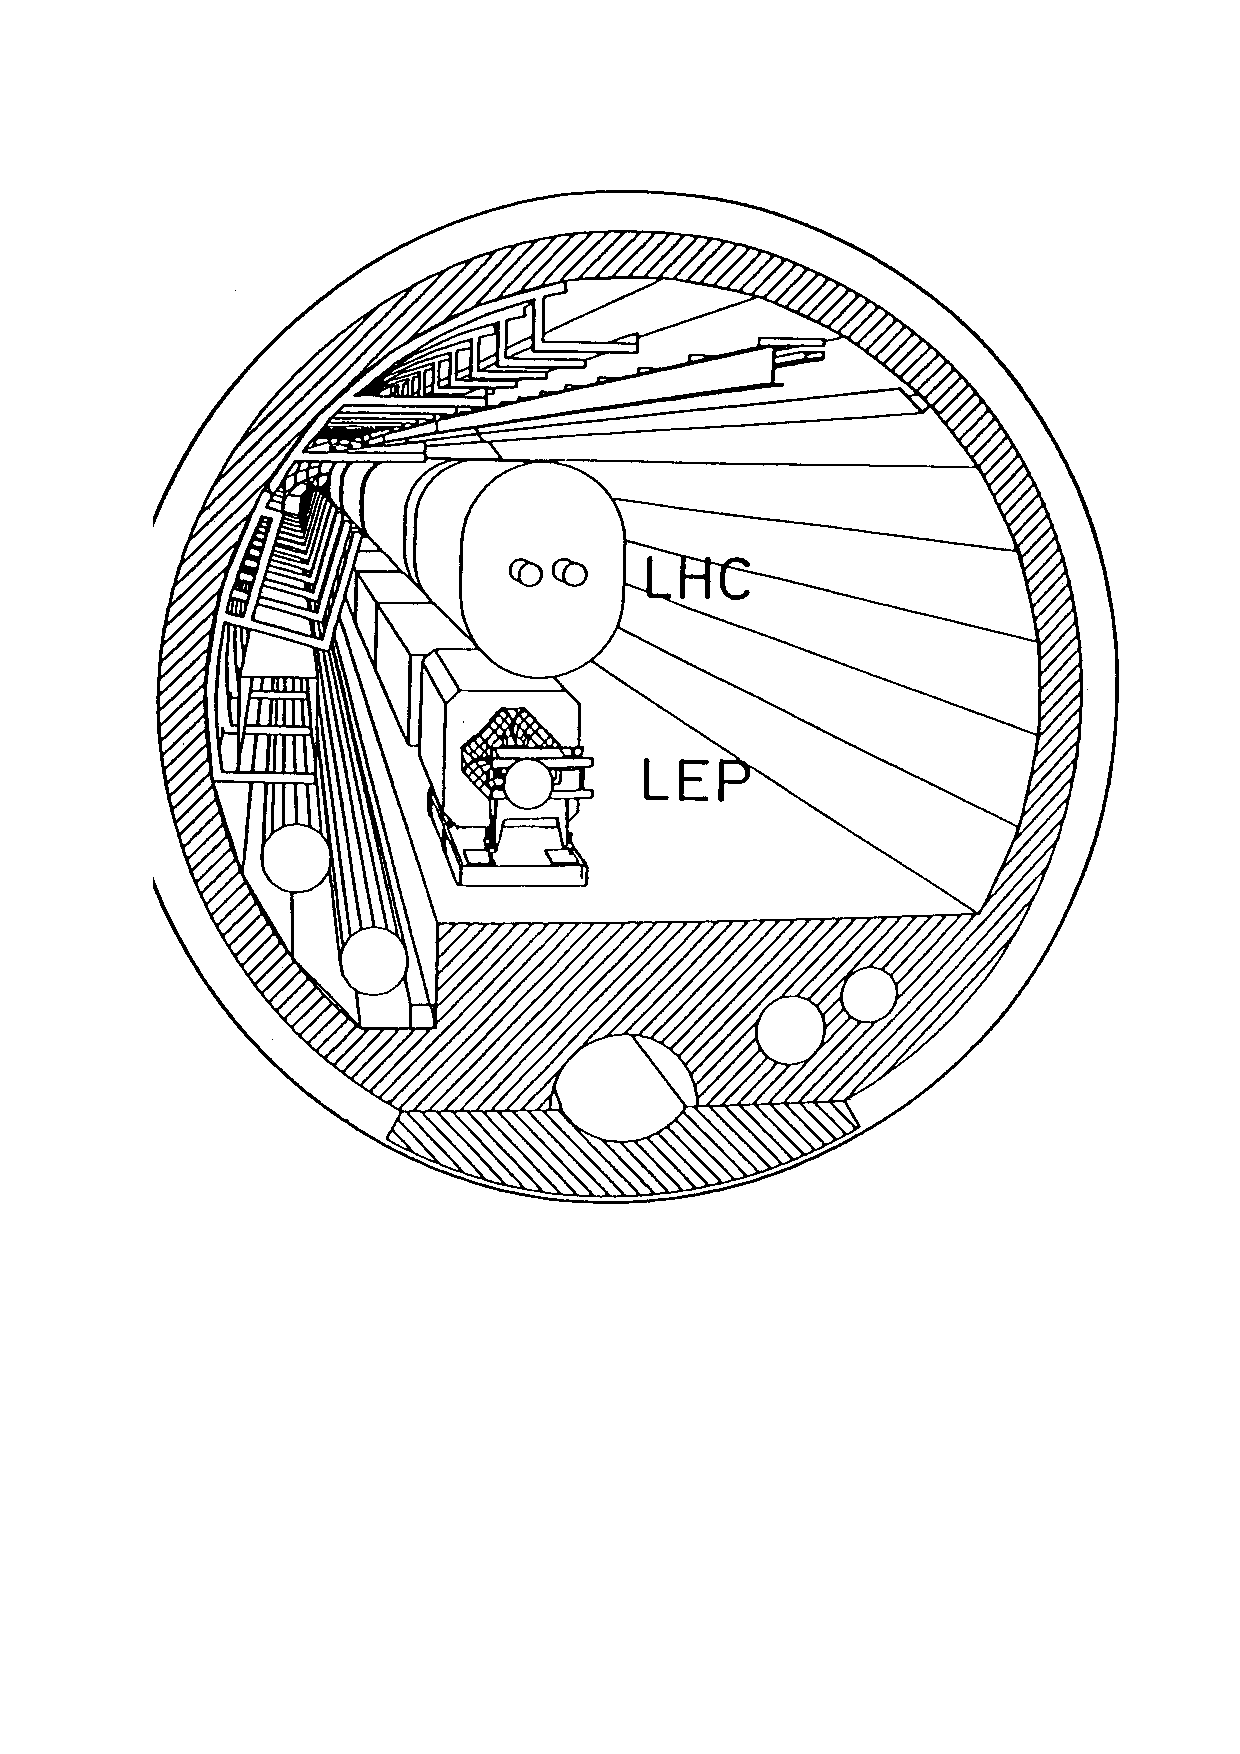
\includegraphics[width=0.8\textwidth]{lep-lhc.pdf}
\label{fig:lhc:lep-lhc}
\caption{A schematic drawing of the initial design of a shared LEP/LHC tunnel, with the LHC beamline positioned on top of the existing LEP beamline~\cite{ECFA1984}.}
\end{figure}

%%%%%%%%%%%%%%%% 

With the approval of the SSC in 1987 and the subsequent start of construction in 1991, CERN was mostly focused on the construction and operation of LEP but did not stop planning for the LHC. This proved remarkly prescient, as in the face of changing budget priorities and the end of the Cold War, the SSC ended up being cancelled in 1993. \editnote{This probably needs citations.} CERN, on the other hand, approved a staged construction plan for the LHC in 1994, targetting first 10~\TeV~collisions in 2004 and then a higher energy in 2008. \editnote{Statement about internation collaboration, compared to SSC? Statement about the 10 TeV plan being dropped?}

The Conceptual Design Report~\cite{LHCCDR} published in 1995 reflected the changed landscape with the demise of the SSC and the results of more detailed cost estimates. The design energy was lowered to 14~\TeV-- higher energies would have required more costly magnets-- while the design luminosity was actually increased to 10$^{34}$~\lumirate. This increase in luminosity came at a cost: the number of interaction points was reduced to four instead of eight, and only two would receive collisions at a high rate. \editnote{Mention pileup here or no?} Critically, it was also decided to remove the LEP beamline and magnets, as it was deemed too costly to follow the existing LEP infrastructure. While this reduced the physics program of the LHC, being the only high energy hadron collider was still a rather broad portfolio. For budgetary reasons, the initial proposal was for a two-stage design, with the first stage operating with only two-thirds the dipoles and therefore a lower energy.

Non-member states joined the proposal quickly: Japan contributed in 1995; India, Russia, and Canada joined in 1996; and the US became a partner in 1997. This financial outlook for the LHC was still not completely safe, as Germany (and later the UK) unilaterally reduced their contribution to CERN between 8-9$\%$. This issue was resolved by allowing CERN to take on debt to finance the entire project in one construction phase-- a decision which raised the total cost of the LHC by $20\%$.


With the shutdown of LEP in 2001\footnote{Not without controversy, as there was perhaps a tantalizing sign of an excess in Higgs-boson like events during the final runs of LEP.\editnote{cite me}}, the construction of the LHC began in earnest. It would take till 2007 to install the last magnet in the LHC, and the detectors finalized their own installations only in 2008. Figure~\ref{fig:lhc:lhc-tunnel} shows the final state of the LHC tunnel (without the originally planned LEP beamline). The first low-energy collisions occured on September 10, 2008, putting the LHC almost on track of its initial goal of 14~\TeV collisions in 2008. \editnote{Probably want to add a bit more on construction.}

%%%%%%%%%%%%%%%%

\begin{figure}
\centering
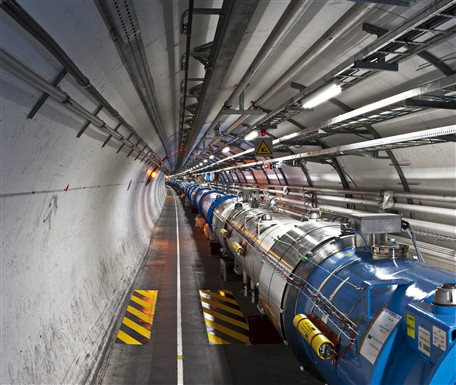
\includegraphics[width=0.8\textwidth]{lhc-tunnel.jpg}
\label{fig:lhc:lhc-tunnel}
\caption{A photo of the final LHC tunnel, no LEP beamline, in contrast to the first plans shown in Figure~\ref{fig:lhc:lep-lhc}. Photo courtesy of USLHC.}
\end{figure}

%%%%%%%%%%%%%%%% 

However, an ``incident'' on September 19 ended up delaying the full startup for a year~\cite{Incident}. On that day, the operators were testing the last sector of the LHC at current levels appropriate fo 5.5~\TeV beams. A resistive zone developed in the electrical bus connection between a dipole and quadrupole magnet. While the power supply detected this and shut down within 0.39 seconds and the quench protection circuitry began to engage at 0.89 seconds, it was already too late: an electrical arc had sparked and punctured the liquid helium enclosure and the insulation vacuum along the cryostat. This, along with the electrical noise induced by the power supply shutdown and the heat dissipation caused by the quench protection circuitry, triggered a chain reaction in which several other magnets also began to quench and other vacuum systems were degraded. As the helium began to escape the cryostat, pressure relief valves correctly opened and vented the helium to atmosphere. However, an additional complication proved to be a problem: neighboring subsectors had their vacuum systems separated by vacuum barriers, meant to isolate the vacuum systems of neighboring areas. The vacuum barriers could only sustain a rather low pressure difference, and the extreme pressures generated by the evacuating helium overwhelmed these connections. The attendant large pressure forces ended up displacing dipoles from their support structures, and knocked the cryostats from their support jacks-- in some cases even ripping the anchors from the concrete floor. A total of six tons of helium, five quadrupoles, and twenty-four dipoles were lost in the incident. 

The damage to the accelerator was repaired in 2009, and on November 20, 2009, 450 GeV protons from the Super Proton Synchotron were injected into the LHC for the first time since the incident. November 23rd saw the first $pp$ collisions in all four LHC detectors, albeit at only $\sqrt{s} = 900$~\GeV. Several very short runs at this energy and $\sqrt{s} = 2.36$~\TeV followed, before the first $\sqrt{s} = 7$~\TeV collisions occured on March 30, 2010. It was decided to operate the LHC for several years at this lower energy, as more accelerator upgrades and consolidation would be required to safely operate at $\sqrt{s} = 14$~\TeV. 2010 saw a peak luminosity of only $2\times10^{32}$~\lumirate as the accelerator only very gradually increased the collision rate. 2011 saw delivery at a peak of $4 \times 10^{33}$~\lumirate-- only three times lower than the design luminosity.

After two years of successful and safe operations at the reduced energy, 2012 saw a large increase in luminosity-- to a peak of $8\times10^{33}$~\lumirate-- and an increase of the collision energy to 8~\TeV. The LHC then proceeded to shut down in 2013 until mid-2015 for a further round of repairs and consolidations of electrical connections to guarantee the safety of operations at near the design energy. As the restart of the LHC approaches in the coming months, we are anticipating collisions at 13~\TeV with luminosity likewise reaching near design levels. The LHC will have broken energy records twice in the span of five years, making this an incredibly exciting time to be working in particle physics.


\section{Machine Design}

The LHC is the last of a long chain of accelerators used to accelerate ordinary protons obtained from hydrogen gas\cite{cern-accelerators}. The entire accelerator complex is shown in Figure~\ref{fig:lhc:cern-accelerators}. Protons from a simple bottle of hydrogen gas are stripped of their electrons in an electric field and are injected into the chain at the Linac2, which accelerates the particles to 50 MeV. The Proton Synchotron Booster (PSB) then accelerates the particles to 1.4 GeV, and sends them off to the Proton Synchotron (PS) to be accelerated to 25 GeV. The Super Proton Synchotron (SPS) then accepts the protons and accelerates them to 450 GeV, which is the energy of injection at the LHC. The injection process per beam takes 260 seconds, and then another 20 minutes is required to raise the energy to collision levels.

%%%%%%%%%%%%%%%%

\begin{figure}
\centering
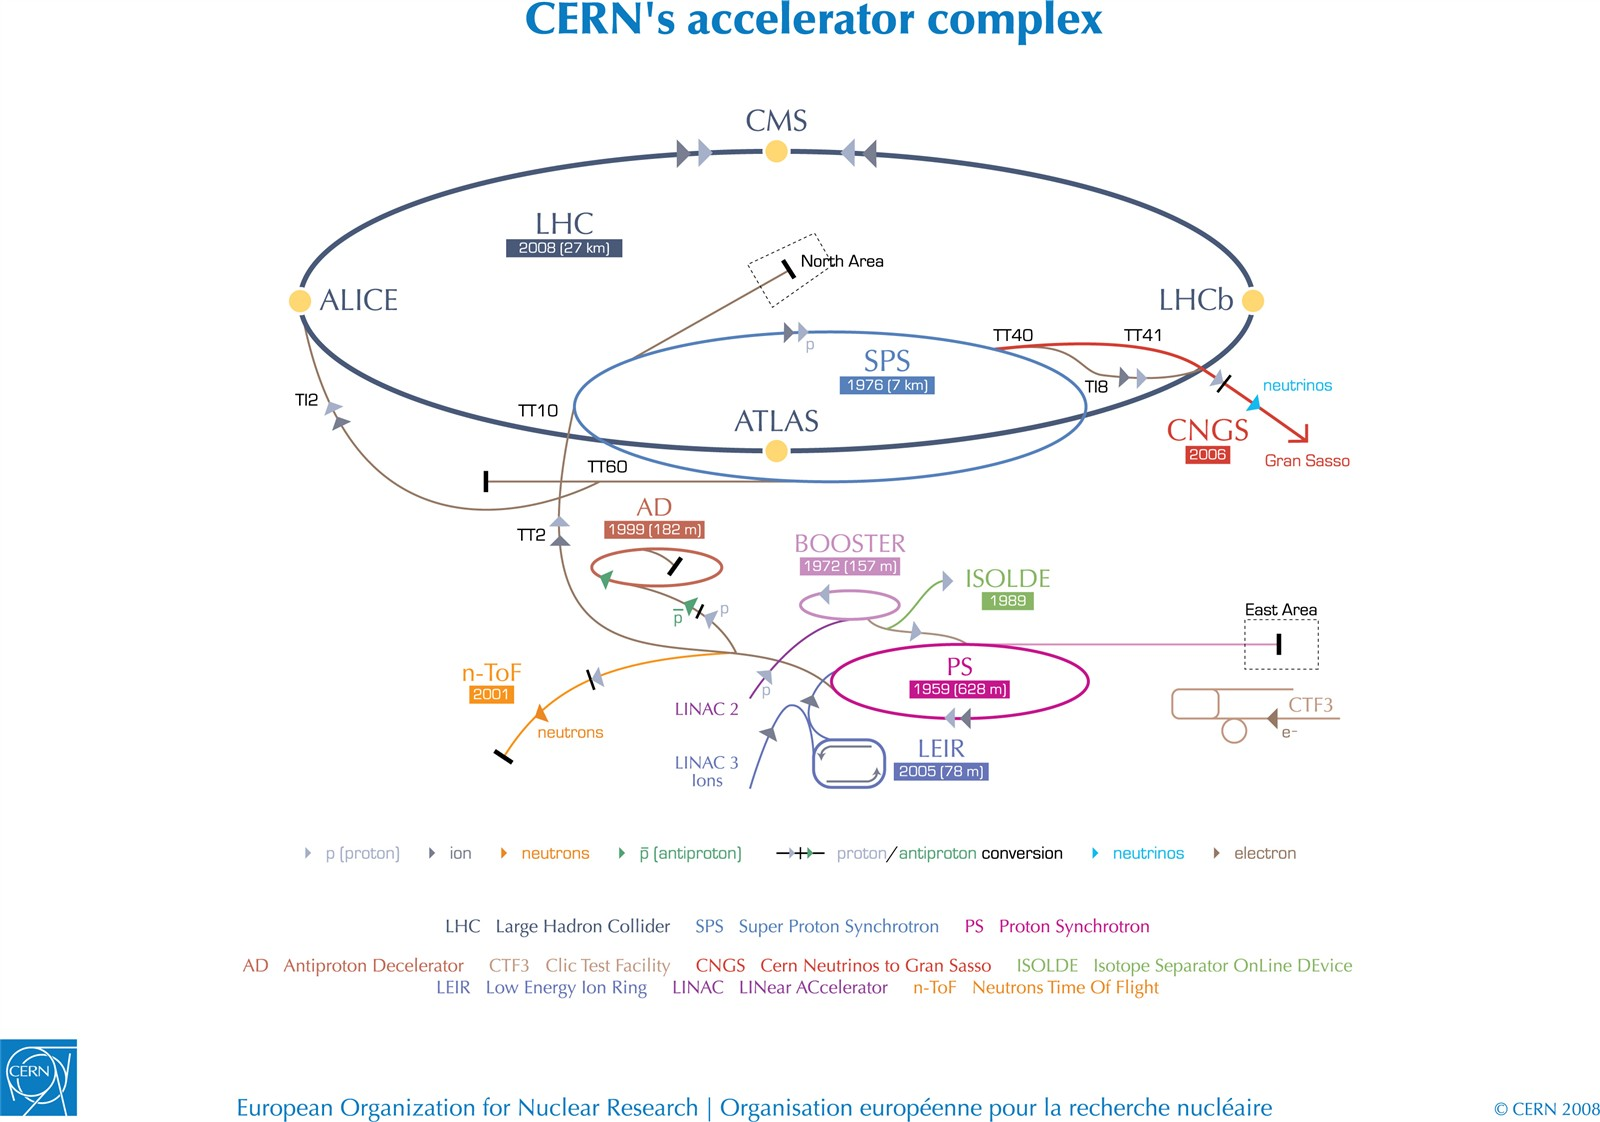
\includegraphics[width=0.8\textwidth]{cernaccelerators.jpg}
\label{fig:lhc:cern-accelerators}
\caption{A diagram of the CERN accelerator chain, with each accelerator listing both its year of completion and length. Copyright CERN.}
\end{figure}

%%%%%%%%%%%%%%%% 

Each stage of the chain accelerates particles by a factor of between 10-20 times their energy. This is a consequence of the fixed bending radius in an accelerator, $\rho$, which is~\cite{accelerator-book}:
%
\begin{equation}
\label{lhc:bending}
\frac{1}{\rho} (\mathrm{m}^{-1}) = 0.2998 \frac{|B (\mathrm{T})|}{\beta E (\GeV)}.
\end{equation}
%
As the bending radius is fixed, this means that as the energy of the beam goes up, the magnetic field must go up linearly to keep the particles inside the ring. This also means that as particles are injected from one accelerator to another (and the radius therefore increases), the magnetic field must be the same factor smaller. The lower range of practical bending magnet strength is set by stray magnetic fields in the earth; the upper range is set by the material of the magnet and energy consumption. These restrictions (how weak the magnets can be during injection, and how strong after acceleration) limit each stage of the accelerator chain to increasing the energy by a factor of $\approx$200. In practice, the accelerating factor is lower (10-20), because it is much easier to not use the full range of the magnet strength (particularly at the low end), and the size of each accelerator is not designed optimally but instead historically, as each accelerator was previously used for collisions at a lower energy. For example, the SPS could have been ejected particles at a much lower energy and the LHC accepted them by using a lower initial field strength, but as the SPS was already built, the operation of the LHC is simplified by using a higher initial field. \editnote{This might need revision}


The LHC itself is composed of eight essentially identical octants, as shown in Figure~\ref{fig:lhc:ring}. Octant 1 contains the collision point for ATLAS (conveniently located right next to the main CERN campus), and Octant 5 for CMS (located in the middle of the French countryside). Each octant is composed of an `insertion'-- a straight segment used for collisions, cleaning, acceleration, beam dumps, etc., as labelled in Figure~\ref{fig:lhc:ring}-- and one half of an `arc' on either end of the insertion point. Each pair of half-arcs forms a sector, which is the main organizational unit for the machine: each sector is independently powered and shares a continuous cryostat. The ring is composed of 1232 dipole magnets which bend the beam around the ring, and 852 quadruple magnets used for beam focusing. The strength of the dipole magnets limits the energy of the beam, as discussed in Equation~\ref{lhc:bending}, so these magnets are particularly critical to the machine design. They are constructed from Niobium-Titanium wire and operated at a temperature of 1.9 K (provided by superfluid helium cooling) at a strength of 8.3 T, using 11850 A of current. An additional 7000 smaller correction magnets (with sextuple, octupole, etc. configurations) are used to shape the beam. The acceleration of the beam is performed by 8 super-conducting RF cavities per beam, each providing an acceleration gradient of 5 MV/m at 400 MHz. 

Operating at full design luminosity, each beam of the LHC contains 2808 bunches each filled with $10^{11}$ protons. This corresponds to a bunch spacing of 25 ns, with longer spacing in between so-called ``bunch trains'': the exact structure of the fill pattern is determined by the fill patterns of the prior accelerators, and the need to provide gaps which can be used to safely dump the beam if necessary~\cite{lhc-bunches}\footnote{In particular, the size of these gaps is determined by the turn-on time of the LHC beam dump kicker of about 3~$\mu$s.}. In operations in 2010-2012, a minimum bunch spacing of 50 ns was used due to electron-cloud effects restricting the operation at 25 ns; the bunch charge was instead increased to deliver additional luminosity. 

Another important parameter describing the beam conditions is the \textit{emittance} $\epsilon$, defined as an ellipse with:
%
\begin{equation}
\epsilon = \gamma x^2 + 2 \alpha x x' + \beta x'^2
\end{equation}
%
where $\gamma$, $\alpha$, and $\beta$ are the ellipse parameters, and $x$ is a coordinate and $x'$ the velocity of that coordinate~\cite{accelerator-book}. The overall emmittance $\epsilon$ is conserved by Liouville's theorem, but focusing magnets can change the other parameters of the ellipse. In particular, as $\beta$ shrinks and $\gamma$ grows, the physical size of the beam in that direction becomes smaller, but with a wider range of velocities. Thus at interaction points, $\beta$ is minimized such that the transverse size of the two beams are minimized and collisions are most likely. This particular value is called $\beta^*$, and is a key parameter in describing the luminosity of the accelerator. Note that in principle each transverse coordinate can have indepedent sizes, but typically circular beams are assumed.

%%%%%%%%%%%%%%%%

\begin{figure}
\centering
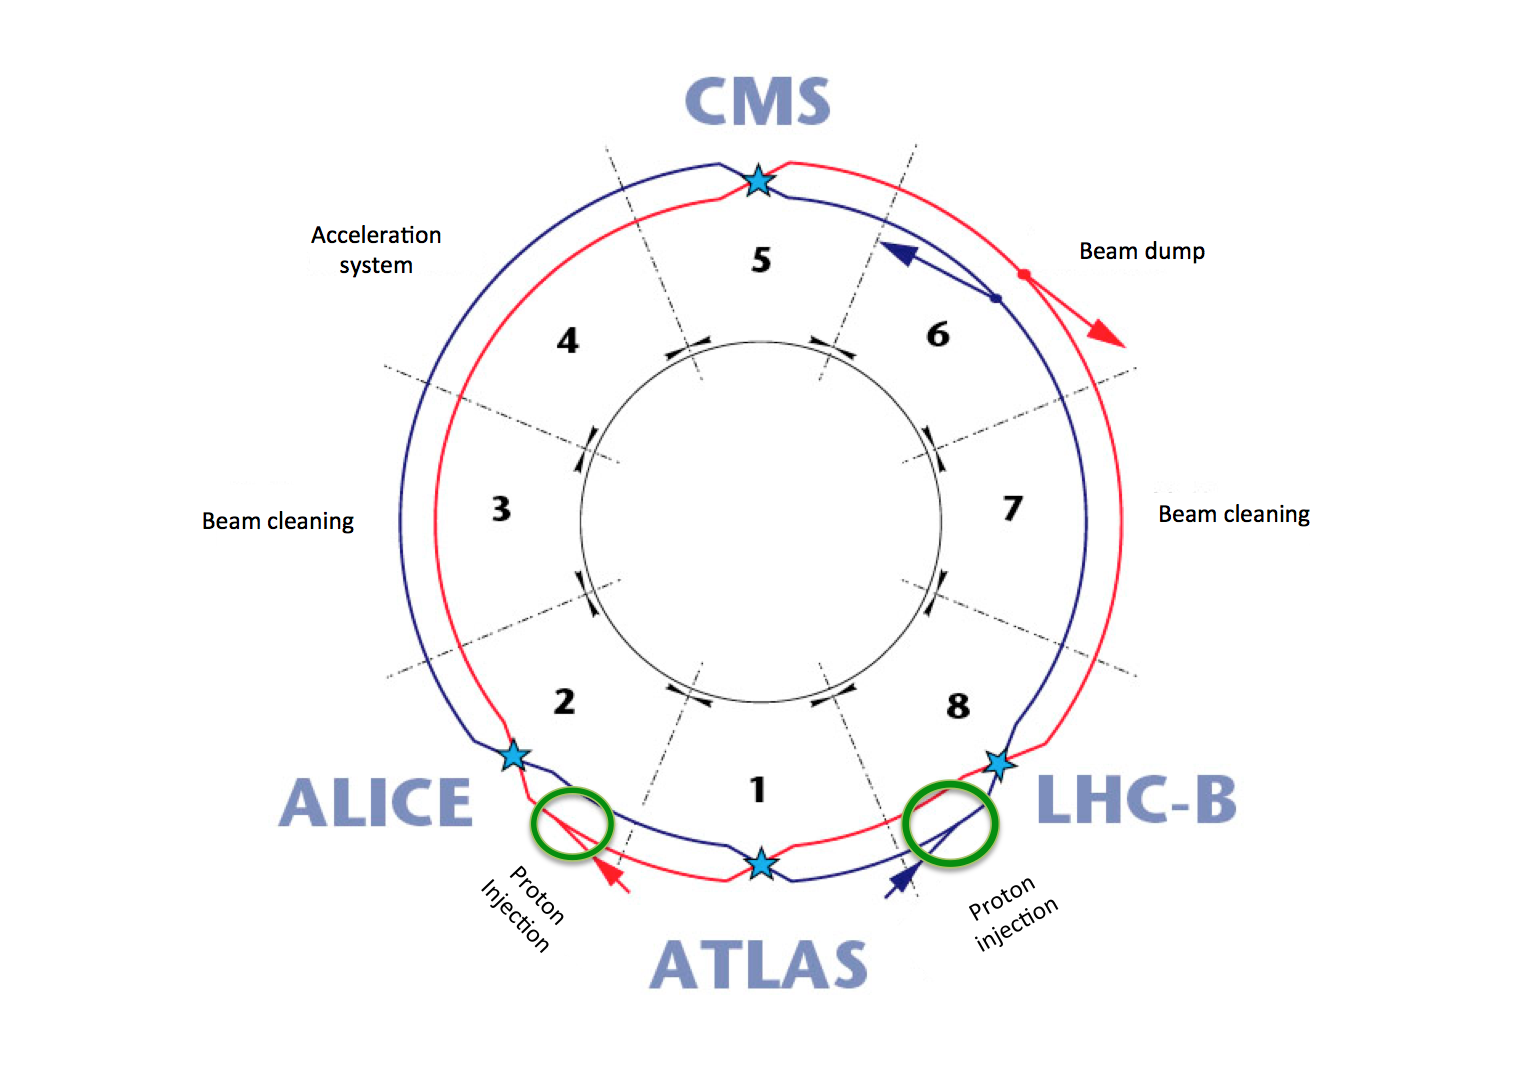
\includegraphics[width=0.8\textwidth]{ring.png}
\label{fig:lhc:ring}
\caption{A diagram of the CERN accelerator chain, with each accelerator listing both its year of completion and length. Copyright CERN.}
\end{figure}

%%%%%%%%%%%%%%%% 

\section{Luminosity, and Pileup}
\label{lhc:luminosity-and-pileup}

Assuming the beams are circular, all of the previously discussed beam parameters come together in defining the luminosity:
%
\begin{equation}
\mathcal{L} = \frac{N^2 k_b f \gamma}{4\pi \epsilon_n \beta^*} F
\end{equation}
%
where $N$ is the number of protons per bunch, $k_b$ is the number of bunches per beam, $f$ is the revolution frequency, $\gamma$ is the relativistic factor, $\epsilon_n$ is the normalized emittance, $\beta^*$ is the $\beta$ value at the IP, and $F$ is a geometric factor indicating the crossing angle of the beams. This shows clearly the handles that the accelerator operators have to increase the luminosity: they can increase the number of protons and the number of bunches, or decrease the size of the beam.

Luminosity is a measurement of the rate of collisions; the \textit{integrated luminosity} refers to the amount of data collected over a period of time. Luminosity is typically reported in units of \lumirate, which is an inverse cross-section per time. Another commonly used unit is the \textit{barn}, which is $10^{-24}$ cm$^2$. Luminosities in ATLAS are typically reported in \ipb~or \ifb. The product of the integrated luminosity and the cross-section of production for some physics process ($pp \rightarrow t\bar{t}$, $pp \rightarrow \tilde{g}\tilde{g}$, etc.) gives the number of events expected for that process in that amount of data.

Increasing the number of bunches (which is possible by switching from 50 ns bunchspacing to 25 ns, for example) increases the frequency of bunch crossings, but does not increase the rate of collisions per bunch crossing. The other factors do the opposite: they keep the rate of bunch crossings constant, but increase the rate of collisions per bunch crossing. Historically in hadron colliders, the expected number of collisions per crossing has been very low, and often less than 1. With the extremely strong performance of the LHC, however, the rate of collisions per crossing has increased to significantly more than one, leading to the condition of \textit{pileup}.

As the expected rate of bunch-crossings is 400 MHz-- far higher than what the detectors can record-- a triggering system is typically used to quickly identify ``interesting'' events for read-out and future analysis. The rate of interesting events is much lower than that of the full interaction cross-section, so there is typically only one interesting event per bunch crossing (at most). This means that when an interesting event is recorded, it is embedded in a background of other collisions, referred to as pileup. The LHC is the first collider which has to deal with significant levels of pileup, as it was not feasible to use an even lower bunch-spacing, leaving only increasing the per-bunch collision rate to increase the overall luminosity.

The pileup profiles-- defined using the variable $\mu$, or the average number of collisions per bunch-crossing-- for 2011 and 2012 operations is shown in Figure~\ref{fig:lhc:mu-profile}. $\mu$ is an average variable which describes the beam conditions-- the actual number of interactions per bunch-crossing can fluctuate with Poisson statistics, and is better measured with variables like $N_{vtx}$, the number of reconstructed primary vertices using the tracking detectors. The wide distribution of $\mu$ values is due to two effects. First, the operation of the accelerator is optimized throughout the year, leading to lower values of $\beta^*$ and higher $N$ and $k_b$, and thus changing $\mu$ over time. Additionally, the expected $\mu$ can change during a run-- in particular, as collisions occur and the number of protons in a bunch decreases over time, $\mu$ will decrease proportionally.

%%%%%%%%%%%%%%%%

\begin{figure}
\centering
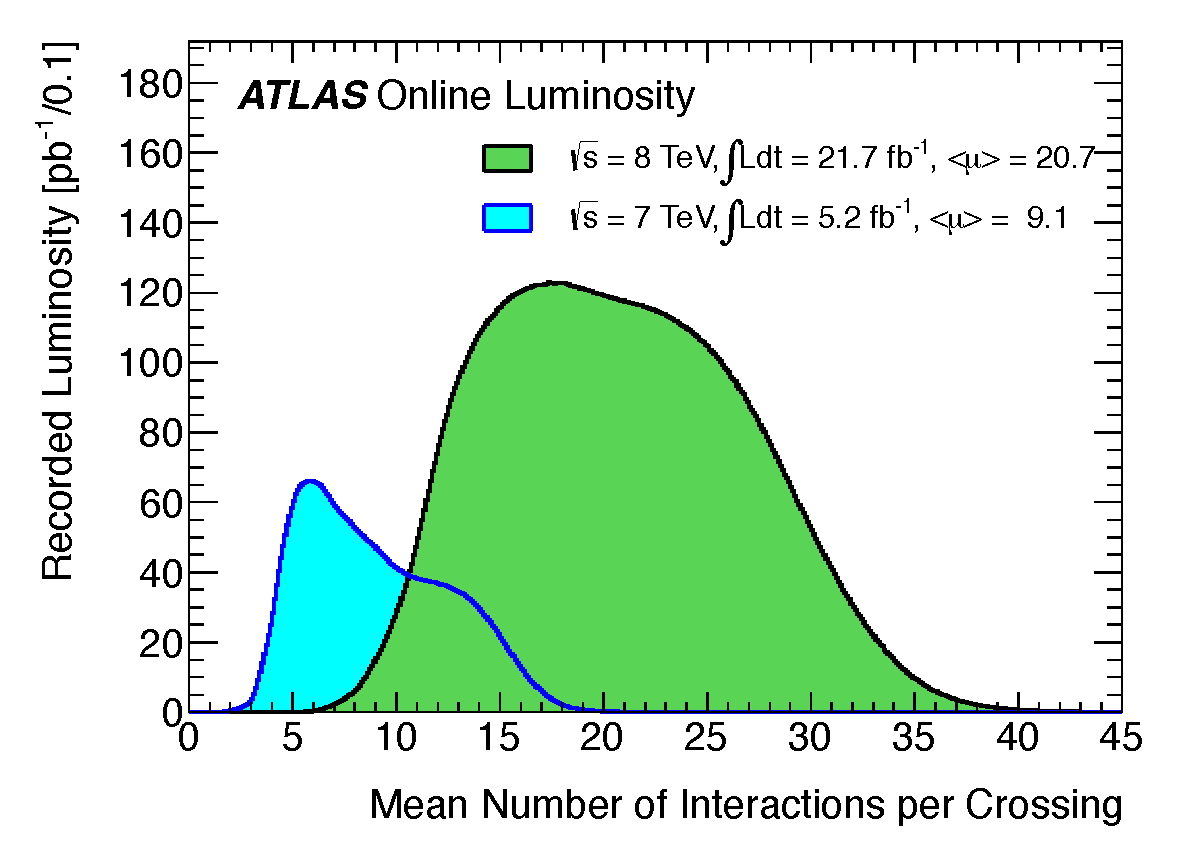
\includegraphics[width=0.7\textwidth]{mu_2011_2012-dec.pdf}
\label{fig:lhc:mu-profile}
\caption{The profile of the average number of interactions per bunch crossing, $\mu$, delivered during operations in 2011 and 2012.}
\end{figure}

%%%%%%%%%%%%%%%% 


\section{Operations in 2010-2012}

Operations during Run 1 of the LHC were extraordinarly successful: in 2010, the collider delivered 48.1 \ipb to ATLAS, 5.46 \ifb in 2011, and 22.8 \ifb in 2012. Figure~\ref{fig:lhc:lumivsyear} shows the integrated luminosity delivered as a function of time, demonstrating the remarkable advances in collision rate as accelerator operations became more advanced. Table~\ref{tab:lhc:parameters} shows the typical beam parameters in each year of operation, compared to the design. In some respects-- emittance and proton number-- the LHC is actually outperforming the design specifications, which has led to very high luminosity levels even with a 50 ns bunch spacing. This comes at the price of the much higher than expected pileup levels, and the correponding difficulties in detector operation that this creates.

%%%%%%%%%%%%%%%%

\begin{figure}
\centering
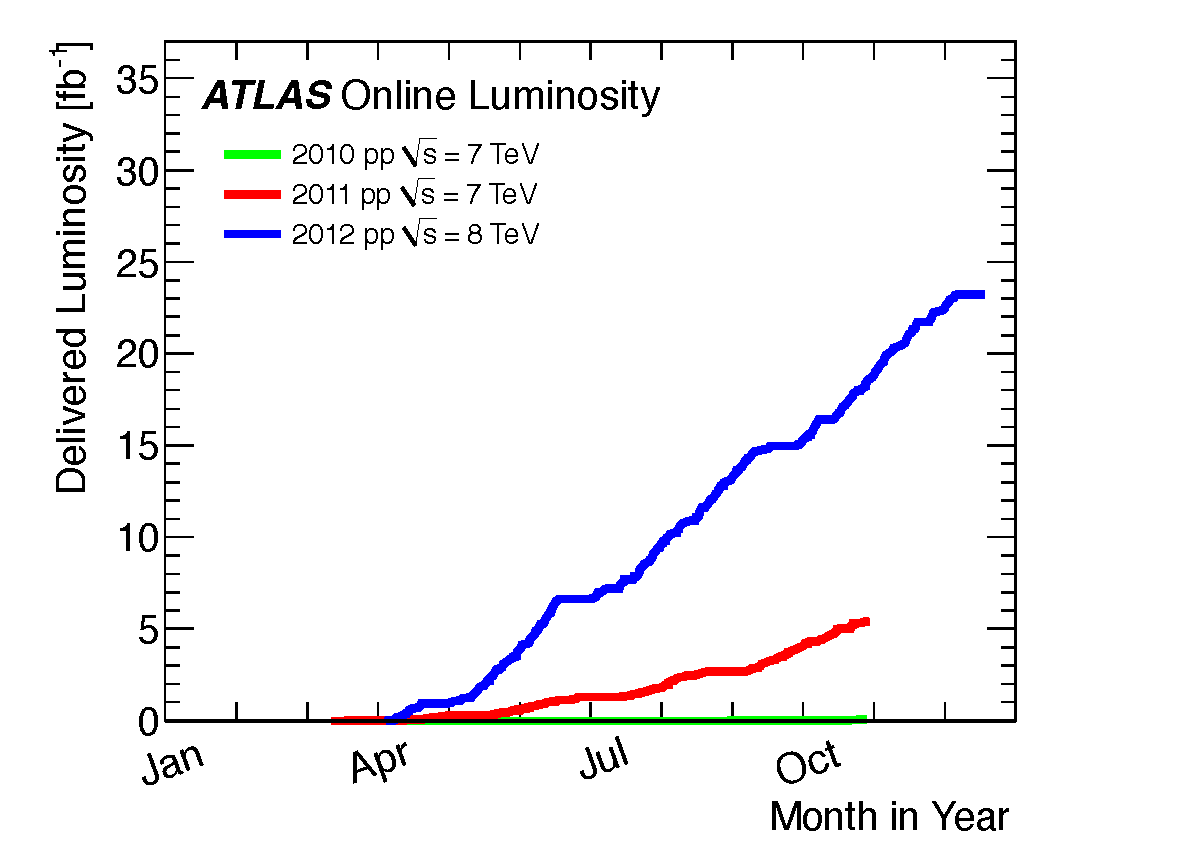
\includegraphics[width=0.7\textwidth]{intlumivsyear.pdf}
\label{fig:lhc:lumivsyear}
\caption{The integrated luminosity as a function of time in Run 1, as measured by the ATLAS detector.}
\end{figure}

%%%%%%%%%%%%%%%% 

\begin{table}
	\caption{Table of LHC run parameters in Run 1, and the design.}
	\label{tab:lhc:parameters}
	\begin{center}
		\begin{tabular}{l|cccc}
		\hline

		\hline
		\textbf{Parameter} & \textbf{2010} & \textbf{2011} & \textbf{2012} & \textbf{Design} \\
		\hline
			 Beam Energy [TeV] & 3.5 &        3.5    &       4.0 &            7.0\\
			 $\beta^*$ [m]      & 2.0/3.5 &     1.5/1.0   &       0.6 &            0.55\\
			 Bunch spacing [ns] & 150 &         75/50   &       50 &             25\\
			 Number of bunches  & 368 &         1380    &       1374 &           2808\\
			 Average proton number  & 1.2 $\times 10^{11}$ &    1.45 $\times 10^{11}$     3.5    &   1.7 $\times 10^{11}$ &     1.15 $\times 10^{11}$\\
			 Normalized emittance at start of fill [mm.mrad]  & 2.0 &    2.4 &      2.5    &   3.75\\
			 Peak luminosity [\lumirate] & $2.1\times 10^{32}$   &  $3.7 \times 10^{33}$   & $7.7 \times 10^{33}$ & $1 \times 10^{34}$ \\
			 Maximum $\mu$ &  4  &  17   &  40 & 19 \\
		\hline

		\hline
		\end{tabular}
	\end{center}
\end{table}

Figure~\ref{fig:lhc:lumivstime} shows the peak luminosity as a function of time in Run 1, and Figure~\ref{fig:lhc:muvstime} shows the peak pileup rate during the same period. In particular, it is clear that the growth is directly related: almost the entirety of the luminosity gain seen in 2011 and 2012 came at the price of increased pileup.

%%%%%%%%%%%%%%%%

\begin{figure}
\centering
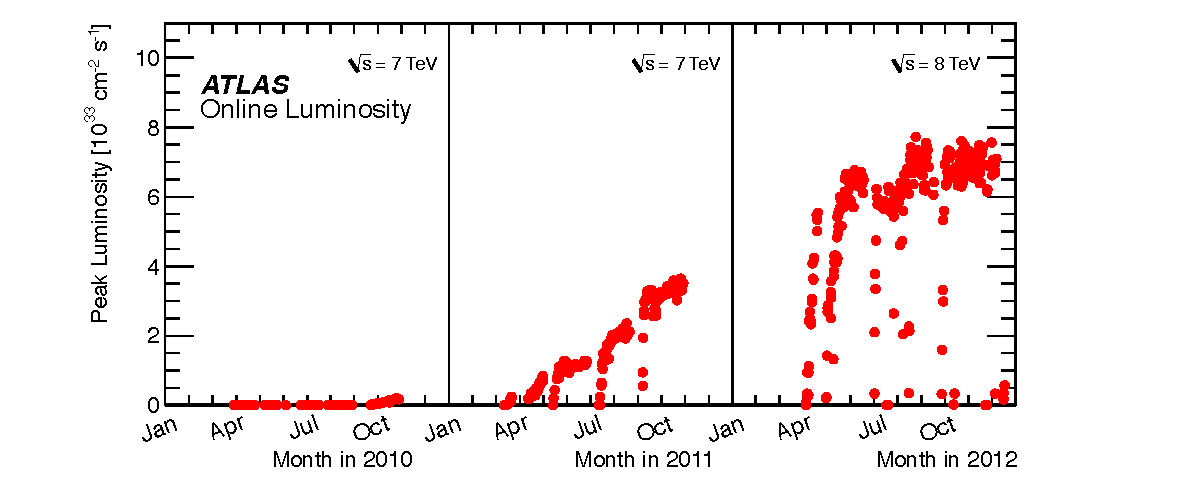
\includegraphics[width=0.7\textwidth]{lumivstime.pdf}
\label{fig:lhc:lumivstime}
\caption{Peak luminosity delivered by the LHC as a function of time in Run 1, as measured by the ATLAS detector.}
\end{figure}

%%%%%%%%%%%%%%%% 


%%%%%%%%%%%%%%%%

\begin{figure}
\centering
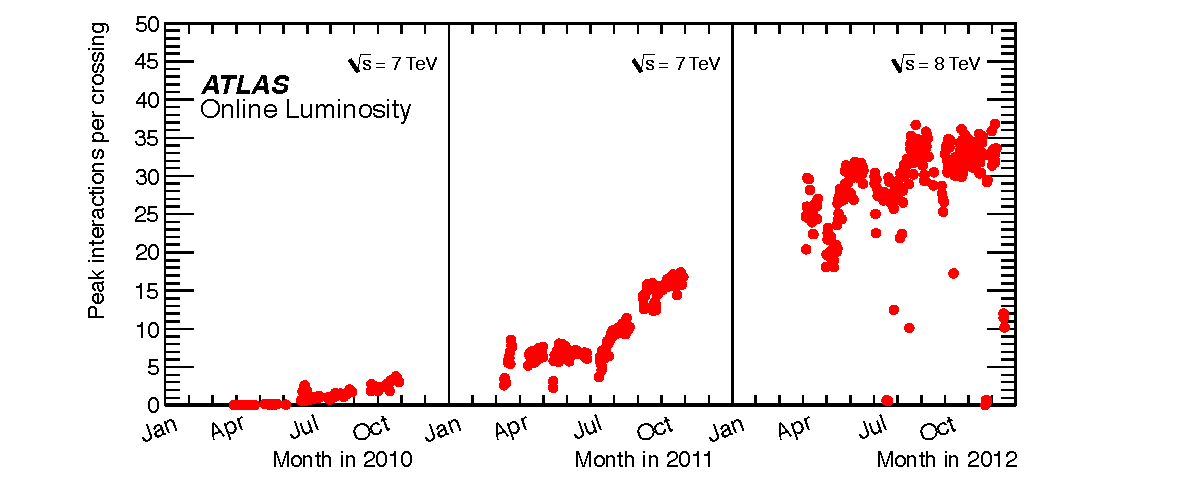
\includegraphics[width=0.7\textwidth]{muvstime.pdf}
\label{fig:lhc:muvstime}
\caption{Peak interactions per crossing as a function of time in Run 1, as measured by the ATLAS detector.}
\end{figure}

%%%%%%%%%%%%%%%% 


